\section{Introduction}


Recent advances in nano- and biotechnology have brought a great deal of interest to the dynamics and structure of polynucleotides such as DNA. To understand the complex properties (such as self-assemblance), a good model of DNA is essential. The inherently large complexity of DNA molecules and their interactions, however, renders it difficult to find a simple theoretical model that is able to encompass all observed phenomena and complex behaviour of DNA. This is where computer simulations come in.\footnote{A review of current numerical simulation methods can be found in Slater \etal \cite{slater2009modeling} For a review of molecular dynamics methods for biophysics, see Karplus \& McCammon \cite{karplus2002molecular} and a recent overview specifically regarding molecular dynamics simulations of DNA can be found in P\'erez \etal\cite{perez2011frontiers}}

Depending on the behaviour that one tries to simulate, different levels of detail are needed. To investigate the smallest phenomena, a simulation of all the atoms in the molecule (and possibly the solvent) is needed. This is for instance the case when one wants to examine the precise role of active sites in enzymes \cite{weiner1986all}.  However, such simulations are computationally extremely expensive to run. For example, the microsecond simulation time barrier has only recently been broken, and that was for a dsDNA of only 12 nucleotides \cite{perez2007dynamics}.

To investigate macroscopical quantities, it often suffices to use a very coarse model of the actual DNA where lots of monomers are combined into a single entity. For instance, a popular model is that of a (self avoiding) random walk. Simulating such coarse-grained models is computationally cheap and can be done for very long timescales \cite{elber2005long}.

Concerning `coarseness', the model we use will be somewhere in between. It uses the three-sites-per-nucleotide (3SPN) approach due to Knotts, Rathore, Schwartz \& De Pablo \cite{knotts2007coarse} (called the 3SPN.0 model). It reduces the complexity of a nucleotide to three interaction sites (sugar, base, phosphate). The parametrization of that model was done by fitting it to experimental data of DNA-melting behaviour between 260--400\,K. An update to this model by the same group (Sambriski, Schwartz \& De Pablo \cite{sambriski2009mesoscale}) extends this model to also take into account the properties of the solvent (3SPN.1 model).

In 2011, Florescu \& Joyeux \cite{florescu2011thermal} further extended this model by slightly adjusting the interactions and contribution of the base pairing which gives better and more precise results for the denaturation of long DNA strands. This model (called the 3SPN.2 model from now on) thus gives a computationally cheap way of simulating the double helix structure of a DNA molecule, with experimentally fitted parameters that are available in the literature.



\subsubsection*{Goal}

We want to use this 3SPN model to research the effects of different loop structures (loop size, length of the complementary stem, \ldots) on interesting DNA behaviour, namely re/denaturation (`zipping/unzipping') and hairpin formation (the zipping of a single DNA strand with complementary base pairs, separated by a loop of non-complementary base pairs, as illustrated in Figure \ref{hairpin_example}).
\begin{figure}[h]
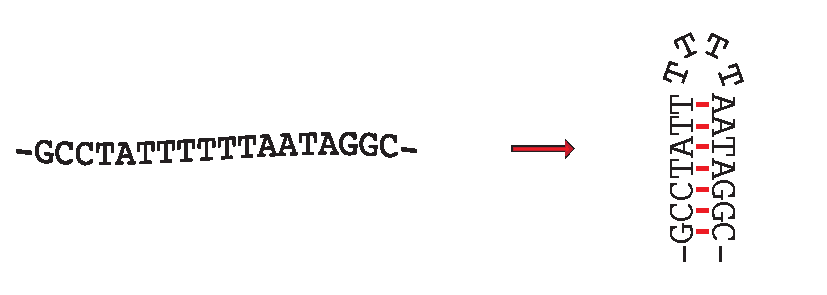
\includegraphics{images/hairpin_example}
\caption{Example of a hairpin formation.}\label{hairpin_example}
\end{figure}
We wrote a custom implementation of the 3SPN model with emphasis on performance, using the technique of spacial partitioning \cite{plimpton1995fast} to improve the performance of the (short ranged) nonbonded interactions.

The model will be used to investigate the scaling dynamics of the zipping and unzipping times of DNA hairpins with varying stem length. The formation of such hairpins in single stranded DNA has been shown to be very relevant for gene expression \cite{oettinger2000hairpins}. It has also been shown that hairpin formation is closely linked to translocation of DNA through nanopores \cite{carlon2011anomalous}. Hence, it is certainly relevant to have a better understanding of hairpin formation.

Previous simulations with a highly simplified Monte Carlo `zipper' model (Ferrantini \& Carlon \cite{carlon2011anomalous}) show a behaviour of the characteristic zipping time $\tau \sim S^{1.37(2)}$ and an unzipping time $\tau \sim S$ with $S$ the stem length of the hairpin. At the equilibrium temperature, the characteristic timescale scales as $\tau \sim S^{2.26(2)}$ \cite{walter2011fractional}. However, that model did not take into account the inherent twisting of the stem that has to occur due to the helical nature of double stranded DNA.

Simplified Poland Scheranga models that have added constraints to the moves to locally preserve the DNA helicity predict scaling laws of $\tau \sim N^{\beta}$ for $\beta \approx 3$ and $N$ the number of base pairs \cite{baiesi2009multiple}.
Slightly more complicated models of DNA denaturation that involve Monte Carlo moves on a grid and also preserve helicity, predict scaling exponents of $\beta = 2.57(3)$  \cite{carlon2010unwinding}.

The 3SPN model, will automatically correctly represent these structural properties of a DNA hairpin and we will examine whether this changes the scaling behaviour. 

Furthermore, because we will use a molecular dynamics simulation instead of a Monte Carlo algorithm, it will be possible to extract not only the scaling law, but also the actual pre-factors. These can be used to compare with experimental values to verify the correctness of the model. To the best of our knowledge, however, there is no experimental evidence to date that describes this scaling behaviour with varying stem length. Hence, the result of the model is a prediction.

On the other hand, the scaling with varying loop length (and composition) has received more experimental attention \cite{bonnet1998kinetics}. We will investigate the behaviour of 3SPN model in this regime as well, although we suspect that there will be deviations due to the coarseness of the model. We especially expect deviations for small loop sizes due to the hydrophobic interactions that are unaccounted for. Indeed, it is currently assumed \cite{vallone1999melting, shen2001loop} that these are responsible for deviations at small loop sizes. Nonetheless, it is interesting to see how the 3SPN model behaves in these circumstances, and how it compares to experiment.

In summery, we will use the 3SPN model to simulate a number of biophysical observables and processes that are not yet simulated with this model. We expect that the computational efficiency of the coarse grained model will be a significant advantage of the 3SPN model when simulating scaling behaviour, while still retaining a high degree of morphological accuracy.
